\documentclass[10pt]{article}
\usepackage[T1]{fontenc}
\usepackage[utf8]{inputenc}
\usepackage{amsmath,amssymb,amsthm,mathtools}
\usepackage{graphicx,booktabs,microtype}
\usepackage[a4paper,margin=2.35cm]{geometry}
\usepackage[dvipsnames]{xcolor}
\usepackage[colorlinks=true,linkcolor=MidnightBlue,citecolor=MidnightBlue,
urlcolor=MidnightBlue]{hyperref}
\hypersetup{pdftitle={ALD-SC v2: Constructive Spectral Decoding with Finite Prime-Error Gates},
pdfauthor={Lorenzo Moriondo}}
\newtheorem{proposition}{Proposition}
\newtheorem{remark}{Remark}
\newcommand{\ALDSC}{\textsc{ald-sc}}
\newcommand{\R}{\mathbb{R}}
\newcommand{\Lf}{L_F}
\newcommand{\Uq}{U_q}
\newcommand{\ed}{\lambda^{\mathrm{ED}}}
\newcommand{\diag}{\operatorname{diag}}
\newcommand{\E}{\mathbb{E}}
\newcommand{\MSE}{\operatorname{MSE}}
\newcommand{\code}[1]{\texttt{\detokenize{#1}}}

\title{\textbf{ALD-SC v2: Constructive Spectral Decoding\\
with Finite Prime-Error Gates}\\[4pt]
\large A frozen feature-graph architecture and controlled\\
encoding and reconstruction experiments}
\author{Lorenzo Moriondo\\
\small tuned.org.uk \quad ORCID: 0000-0002-8804-2963\\
\small \texttt{tunedconsulting@gmail.com}}
\date{21 November 2026 \quad Software version 2.0.0}

\begin{document}
\maketitle

\begin{abstract}
ArrowSpace Latent Diffusion with Spectral Chart Conditioning (\ALDSC)
combines a spatial variational autoencoder with a frozen feature-space
graph and a compact spectral chart. Version 2 makes the graph a constructive
part of decoding: learned activations are projected onto graph eigenvectors,
weighted by chart-dependent gates and fixed modal gains, and lifted back
into the decoder. We introduce finite prime-error gains motivated by the
Riemann Hypothesis (RH), alongside heat, envelope and Fourier-phase controls.
The motivation is conditional, but the finite prime-power sums, positivity
constraint and numerical experiments require no unproved number-theoretic
assumption. A shared amplitude rule and squared-gain normalisation make the
comparison explicit. We evaluate held-out linear encoding and noisy
reconstruction on a 128-node analytical path graph, with independent
principal-component training data and 32 phase controls. Prime gating
raises smooth-signal mean squared error (MSE) from 0.061151 to 0.061754 but lowers broadband
MSE from 0.684918 to 0.680581; it ranks 29th and 2nd, respectively,
among the prime arm and phase controls. These outcomes establish
regime dependence, not a unique or general prime advantage. A separate
common-clock experiment checks the exact invariance of linear heat
endpoints at equal integrated time. These experiments isolate mechanisms
that can be incorporated into the neural decoder; they are not trained
image experiments or evidence of semantic coherence on an ArrowSpace
corpus. The revision supplies a reproducible test of a finite spectral
design while separating graph geometry, arithmetic modulation and
numerical scheduling.
\end{abstract}

\noindent\textbf{Keywords:} latent diffusion; graph signal processing;
spectral compression; constructive decoding; prime-power error;
matched controls.

\section{Research question and scope}
\label{sec:introduction}

Latent diffusion separates image compression from iterative generation:
an autoencoder maps images into spatial latents, and a denoiser learns
their distribution~\cite{rombach}. \ALDSC\ asks whether reconstruction
can also exploit a feature-space graph fixed from corpus statistics.
The spatial latent preserves local information; the graph supplies
directions along which a decoder can reconstruct; and a dispersion
descriptor controls allocation among those directions. This is a
structural hypothesis about a decoding operator, not merely a proposal
to append additional metadata to a conventional network.

The present revision adds a precisely specified family of fixed modal
gains to that architecture. The prime-error arm is derived from the
finite fluctuation of the Chebyshev prime-power function. Its mathematical
motivation is the RH scale of relative prime error, but no part of the
implementation assumes RH to be true. An envelope-only arm tests the
asymptotic shape without arithmetic detail, while Fourier phase controls
preserve the discrete spectral magnitudes of the sampled prime waveform.
All arms use a common amplitude scale chosen before outcomes are observed.

Three questions require separate evidence. First, does a smooth graph
basis encode a graph-smooth population efficiently at a fixed coefficient
count? Second, does a particular redistribution of modal gains improve
noisy reconstruction relative to heat attenuation at matched noise
transmission? Third, can a shared change of diffusion time alter an exact
heat endpoint when total integrated time is held fixed? The first two
questions are measured on synthetic signals; the third has a direct
negative theorem and a numerical check. None is equivalent to demonstrating
better generated images.

The contribution is consequently a versioned constructive decoder and
an auditable evaluation of its linear ingredients. The experiments use
an analytical path graph, not an ArrowSpace graph built from an embedding
corpus. They contain no trained image model, perceptual metric, image
likelihood or semantic benchmark. The broader research hypothesis---better
global image coherence under compression through a frozen feature
manifold---remains a target for subsequent controlled training.

\section{The frozen chart and spatial latent}
\label{sec:architecture}

\subsection{Feature geometry}

Let $\Lf\in\R^{F\times F}$ be a real symmetric positive semidefinite
feature-graph Laplacian. Write
\begin{equation}
 \Lf=U\diag(\nu_0,\ldots,\nu_{F-1})U^\top,\qquad
 0\leq\nu_0\leq\cdots\leq\nu_{F-1},
 \quad \Uq=[u_0,\ldots,u_{q-1}].
 \label{eq:graph}
\end{equation}
Graph spectral filtering uses this eigenbasis to resolve signals into
smooth and rough directions~\cite{shuman}. In the intended ArrowSpace
application, graph nodes correspond to feature dimensions rather than
individual images. The ArrowSpace library is the source of the
corpus-level graph construction~\cite{arrowspace}. Once built, the prior
\begin{equation}
 \mathcal G=(\Lf,\Uq,\nu_{0:q},\ed)
 \label{eq:prior}
\end{equation}
is frozen. The per-feature dispersion vector $\ed$ and the Laplacian
eigenvalues $\nu$ are distinct quantities; their similar historical
notation does not make them interchangeable.

For a feature field $A\in\R^{N\times F}$, define
\begin{align}
 \Pi_q&=\Uq\Uq^\top,\qquad A_\parallel=A\Pi_q,\\
 e_k(A)&=N^{-1}\|Au_k\|_2^2,\qquad
 \widetilde e_k=\frac{e_k}{\sum_{j<q}e_j+\epsilon},\\
 \lambda_k^{\mathrm{chart}}&=\sum_{f=1}^{F}\ed_f U_{fk}^2,\qquad
 c_{\mathrm{spec}}=[\,\widetilde e,\lambda^{\mathrm{chart}},\nu_{0:q}\,]
 \in\R^{3q}.
 \label{eq:chart}
\end{align}
The graph basis defines the reconstruction directions. The chart contains
the image-dependent modal energy and the frozen dispersion allocation.
Because energy discards coefficient signs, this descriptor cannot
reconstruct $A$ by itself. Spatial latents and learned decoder activations
carry the information absent from the energy descriptor.

The term ``2.5-D'' denotes the pair $(z,c_{\mathrm{spec}})$, a spatial
latent plus global spectral information. It does not assert a fractional
manifold dimension, an invertible chart, or a rate in bits. In particular,
a scalar difference of Frobenius norms, used as a dual-space diagnostic in
earlier design discussions, is not itself an encoding matrix or a complete
training representation. Here the operative objects are the spatial
tensor, the feature vector or field, and the explicit projection.

\subsection{Variational encoding and latent diffusion}

The encoder produces a Gaussian spatial posterior and a feature summary:
\begin{equation}
 z=\mu_\phi(x)+\exp\!\left(\tfrac12\ell_\phi(x)\right)\odot\eta,
 \qquad \eta\sim\mathcal N(0,I),\qquad A=E_\phi^A(x).
 \label{eq:vae}
\end{equation}
This is the usual variational reparameterisation~\cite{kingma}.
The implemented feature head uses global average pooling followed by
a learned linear projection, giving $A\in\R^{B\times F}$ for a batch
of $B$ images. Equations~\eqref{eq:chart} apply with one feature location
per image. A spatially resolved $N>1$ field is a generalisation, not a
description of the current encoder.

Diffusion acts only on $z$. With a common scalar noise schedule,
\begin{equation}
 z_t=\sqrt{\bar\alpha_t}\,z_0+
       \sqrt{1-\bar\alpha_t}\,\varepsilon,\qquad
 v_t=\sqrt{\bar\alpha_t}\,\varepsilon-
       \sqrt{1-\bar\alpha_t}\,z_0.
 \label{eq:diffusion}
\end{equation}
A small diffusion transformer~\cite{peebles} predicts
$v_\theta(z_t,t,c_{\mathrm{spec}})$, using chart and time conditioning
through adaptive layer normalisation. The chart is not a second diffused
state. Conditional generation must therefore specify how a chart is
provided, selected or sampled; a fixed chart architecture alone does not
define the marginal distribution of charts.

The training design retains reconstruction, variational and spectral
terms:
\begin{align}
 \mathcal L_{\mathrm{VAE}}={}&
 \mathcal L_{\mathrm{rec}}+
 \lambda_{\mathrm{KL}}D_{\mathrm{KL}}(q_\phi(z\mid x)\Vert\mathcal N(0,I))
 +\lambda_{\mathrm{chart}}\|\widetilde e(A)-\widetilde e(\widehat A)\|_2^2
 \nonumber\\[-2pt]
 &+\lambda_{\mathrm{smooth}}
 \frac{\|A(I-\Pi_q)\|_F^2}{\|A\|_F^2+\epsilon},\qquad
 \mathcal L_{\mathrm{diff}}=\E\|v_t-v_\theta(z_t,t,c_{\mathrm{spec}})\|_2^2.
 \label{eq:loss}
\end{align}
Here $\widehat A$ is obtained by re-encoding a reconstruction.
Reconstruction may combine an image-space loss with a separately
configured perceptual loss. These are architecture and training
definitions; the experiments below do not optimise these neural losses.

\section{Constructive decoding in version 2}
\label{sec:decoder}

At a decoder stage, let $H\in\R^{B\times C\times h\times w}$.
Learned maps $P_\ell:\R^C\rightarrow\R^F$ and
$Q_\ell:\R^F\rightarrow\R^C$ connect channel space to the frozen chart.
For one batch element, the implemented operation is
\begin{align}
 a_\ell &=P_\ell\!\left(\operatorname{Mean}_{h,w}H\right),\qquad
 b_\ell=a_\ell\Uq,\\
 g_\ell(c)&=\operatorname{sigmoid}(W_\ell c+b_\ell^{\mathrm{bias}}),\\
 \delta_\ell
 &=Q_\ell\!\left[
  \{b_\ell\odot g_\ell(c_{\mathrm{spec}})\odot d\}\Uq^\top
 \right],\\
 H'&=H+\operatorname{Conv}_\ell\!\left(
  \operatorname{SiLU}\{\operatorname{GroupNorm}
       (H+\operatorname{Broadcast}(\delta_\ell))\}\right).
 \label{eq:block}
\end{align}
The frozen vector $d\in\R^q$ is the v2 modal gain. The learned gate and
fixed gain multiply: replacing one by the other would change the model.
The dispersion vector influences $g_\ell$ through
$\lambda^{\mathrm{chart}}$ in $c_{\mathrm{spec}}$; it is not replaced by
the prime-error waveform.

This is constructive use of the graph because intermediate activations
are explicitly projected, filtered and lifted by $\Uq$. It remains a
hybrid decoder: convolutions and learned feature maps are present, and
the residual path can carry information outside the retained subspace.
Global pooling means the graph branch supplies a spatially broadcast
channel correction, rather than independently filtering each pixel's
feature vector. Those details limit what can be inferred from the phrase
``decoding on the manifold''.

\code{GraphDecoder} applies three such blocks with decreasing channel
width and two spatial upsampling stages. \code{SpectralVAE} requires its
frozen prior at construction and constructs the graph decoder eagerly.
All trainable decoder parameters consequently exist before an optimiser
is created. \code{ModalGate} stores eigenvalues and the selected waveform
as buffers and records the recipe identity in checkpoint state. Heat
is the default recipe; envelope, prime and phase-control recipes are
explicit alternatives with the same parameter count.

The graph block does not replace the variational reparameterisation
in~\eqref{eq:vae}. Reparameterisation enables differentiation through a
latent sample; the graph block specifies a deterministic part of the
conditional reconstruction map. Likewise, despite the historical name
\code{WaveReconstructionBlock}, equation~\eqref{eq:block} is a single
spectral filter step, not a numerical solution of a second-order wave
equation.

\section{Finite prime-error modal gains}
\label{sec:prime}

\subsection{Conditional motivation, unconditional construction}

Define the Chebyshev function using all prime powers,
\begin{equation}
 \psi(x)=\sum_{p^m\leq x}\log p,\qquad
 r(x)=\frac{\psi(x)-x}{x}.
 \label{eq:psi}
\end{equation}
The classical RH error scale is
\begin{equation}
 \mathrm{RH}\quad\Longrightarrow\quad
 \psi(x)-x=O(\sqrt{x}\log^2x),\qquad x\rightarrow\infty.
 \label{eq:rh}
\end{equation}
Classical explicit conditional estimates are given by
Schoenfeld~\cite{schoenfeld}. With $s=\log x$, dividing
equation~\eqref{eq:rh} by $x$ gives the relative scale
\begin{equation}
 r(e^s)=O(s^2e^{-s/2}).
 \label{eq:envelope}
\end{equation}
We use $s^2e^{-s/2}$ as a comparison waveform. We do not assert that
it bounds the finite error with constant one, and do not apply an
explicit conditional bound outside its certified domain. Centring and
normalising this shape further changes its interpretation: the resulting
control is a waveform, not an upper envelope for every sample.

For $q=64$, evaluate $\psi$ on the real grid
\begin{equation}
 s_j=\log16+\frac{j}{q-1}(\log10^6-\log16),\qquad
 x_j=e^{s_j},\quad j=0,\ldots,q-1.
 \label{eq:grid}
\end{equation}
A sieve enumerates primes and all powers no larger than the finite
maximum. Right continuity means a prime power at a grid point is included.
Natural logarithms and float64 arithmetic are used, with the two
grid endpoints explicitly assigned to 16 and $10^6$ to avoid a
log--exponential round trip excluding a boundary prime power. ``Exact finite
prime-power sum'' describes the enumerated set of terms; evaluation of
logarithms and summation still have floating-point error. No zeta-zero
truncation is used to compute this waveform.

\subsection{Matched controls and gain normalisation}

For a nonconstant sampled vector $f$, define
\begin{equation}
 \mathcal S(f)=
 \frac{f-\overline f\,\mathbf1}
 {\sqrt{q^{-1}\sum_j(f_j-\overline f)^2}}.
 \label{eq:standardise}
\end{equation}
The prime arm is $h^{P}=\mathcal S((r(x_j))_j)$ and the envelope arm
is $h^{E}=\mathcal S((s_j^2e^{-s_j/2})_j)$. We generate 32 real Fourier
phase surrogates of $h^P$, preserving the discrete Fourier magnitudes,
the DC component and the Nyquist component. Interior phases receive
independent uniform rotations with the prescribed seed. The resulting
surrogates preserve the mean and root-mean-square (RMS) amplitude up to
round-off. They control the arrangement of the finite waveform, rather
than defining a probability model for the primes.

Across the envelope, prime and all 32 surrogates, select one scale
\begin{equation}
 \beta=\frac{0.25}{\max_{a,j}|h_j^a|},\qquad
 m_j^a=1+\beta h_j^a.
 \label{eq:beta}
\end{equation}
The heat arm uses $m_j^H=1$. Each nonconstant multiplier has mean one,
RMS deviation $\beta$, and lies in $[0.75,1.25]$. There is no clipping
or outcome-dependent selection. An RMS constraint alone would not imply
this amplitude bound; the shared maximum in~\eqref{eq:beta} is essential.

Grid position $j$ is assigned to ascending retained graph mode $j$.
This is an imposed index-to-mode correspondence, not a consequence of
RH. For baseline $d_k^H=e^{-\nu_k}$ at unit heat time, set
\begin{equation}
 \widetilde d_k^a=e^{-\nu_k}m_k^a,\qquad
 d_k^a=\widetilde d_k^a
 \left(\frac{\sum_{j<q}e^{-2\nu_j}}
 {\sum_{j<q}(\widetilde d_j^a)^2}\right)^{1/2},
 \qquad k<q.
 \label{eq:gains}
\end{equation}
Modes $k\geq q$ receive zero in the linear reconstruction experiment.
The neural decoder uses the retained vector $d^a$ within its graph
branch. Changing $q$ recomputes the finite grid and shared scale; gain
families at different ranks are not nested samples of one fixed filter.

\begin{proposition}[Positivity and matched noise transmission]
All retained gains in~\eqref{eq:gains} are positive. Their squared sum
equals $\sum_{k<q}e^{-2\nu_k}$. For isotropic noise
$\xi\sim\mathcal N(0,\sigma^2 I_F)$ and
$K_a=\Uq\diag(d^a)\Uq^\top$,
\begin{equation}
 \E\|K_a\xi\|_2^2=\sigma^2\sum_{k<q}e^{-2\nu_k}.
 \label{eq:noise}
\end{equation}
Moreover $0.6e^{-\nu_k}\leq d_k^a\leq(5/3)e^{-\nu_k}$.
\end{proposition}
\begin{proof}
Every multiplier is positive. Its weighted norm lies between $0.75$
and $1.25$ times the baseline norm, so the final scalar rescaling lies
between $1/1.25$ and $1/0.75$. The gain bounds follow by multiplication.
The norm identity follows directly from~\eqref{eq:gains}; orthonormality
of $\Uq$ then gives~\eqref{eq:noise}.
\end{proof}

The normalisation matches expected transmitted isotropic noise energy,
not total signal energy, wall time, reconstruction quality or the
Lipschitz constant of the full neural decoder. In particular, the final
normalised gains need not be bounded by one. Learned maps, residual
paths and chart-dependent gates also mean that~\eqref{eq:noise} is not
an equal-energy theorem for complete trained networks.

\subsection{Graph waves and arithmetic oscillations}

For a graph wave equation $\ddot y+\Lf y=0$, a nonzero eigenmode has
angular frequency $\sqrt{\nu_k}$. The imaginary part $\gamma$ of a zeta
zero $\rho=1/2+i\gamma$ instead describes oscillation in logarithmic
arithmetic coordinate: a formal relative-error term
$x^{\rho-1}/\rho$ has the factor $e^{-s/2}e^{i\gamma s}/\rho$.
Such terms motivate the distinction between an envelope and a detailed
oscillation, but an infinite explicit formula requires its own
convergence and endpoint conventions.

There is no equality $\gamma=\sqrt{\nu_k}$ in this construction, no
claim that graph modes are zeta zeros, and no deduction of a physical
amplitude bound from RH. The graph supplies an orthonormal basis; a
finite arithmetic sequence supplies an additional design vector.
Any benefit must survive empirical controls and changes of graph,
signal distribution and index mapping.

\section{Common clocks and mode-specific filters}
\label{sec:clock}

\begin{proposition}[Equal-time heat endpoint]
Let $a:[0,T]\rightarrow[0,\infty)$ be integrable, let $\Lf$ be fixed,
and consider $\dot y(t)=-a(t)\Lf y(t)$. Then
\begin{equation}
 y(T)=\exp\!\left(-\Lf\int_0^T a(t)\,dt\right)y(0).
 \label{eq:clock}
\end{equation}
Thus all common scalar clocks with the same integrated time have the
same exact endpoint for every initial state.
\end{proposition}
\begin{proof}
The eigenbasis of $\Lf$ is time-independent. Each coefficient solves
$\dot b_k=-a(t)\nu_k b_k$, so
$b_k(T)=b_k(0)\exp(-\nu_k\int_0^T a(t)\,dt)$. Lifting these coefficients
gives~\eqref{eq:clock}. Equivalently, the time-dependent generators
commute because they are scalar multiples of one fixed matrix.
\end{proof}

Consequently, interpreting the multipliers $m_j^a$ as successive
equal-duration time cells cannot improve an exact unit-time heat
reconstruction: their mean is one. Explicit Euler replaces the exact
transfer by $\prod_j(1-\Delta t\,a_j\nu_k)$ and can produce
clock-dependent errors. These are discretisation effects, not evidence
of an improved continuous-time endpoint. The proposition does not
apply automatically to learned nonlinear denoisers, changing graph
bases, noncommuting operators or genuinely mode-dependent rates.

Equation~\eqref{eq:gains} changes gains across modes and is therefore
a different intervention. A common scalar clock can only yield gains
$e^{-\nu_k\tau}$ for one $\tau$; an arbitrary positive normalised
modulation need not belong to that one-parameter family. It may even
amplify a retained mode relative to one, so interpreting every modal
gate as positive-time heat evolution would be incorrect.

The existing \code{SpectralSchedule} must also be read carefully. Its
formula $\tau_k(t)=\nu_k t$ with $\tau_{k,\max}=\nu_k T$ gives
\begin{equation}
 \bar\alpha_k(t)=
 \cos^2\!\left(\frac{\pi}{2}\frac{\tau_k(t)}{\tau_{k,\max}}\right)
 =\cos^2\!\left(\frac{\pi t}{2T}\right),\qquad \nu_k>0.
 \label{eq:cancellation}
\end{equation}
The common expression provides the continuous extension at $\nu_k=0$.
All modes cross a given attenuation level at the same external time.
Weighting a stopping statistic by $\nu_k$ does not restore distinct
mode schedules:
$\sum_k\nu_k\bar\alpha_k(t)=\bar\alpha(t)\sum_k\nu_k$ depends only
on time and the frozen spectrum. It is not a measured posterior
minimum mean-squared error or a data-dependent convergence certificate.
The optional clock-gated graph decoder averages these attenuations,
giving a common tempo factor. The v2 fixed modal gains supply the
explicit mode-specific allocation studied here.

A related entropy identity is valid under a narrower assumption.
If an individual Gaussian coefficient has variance
$w_ke^{-2\nu_k t}$ with $w_k>0$, its differential entropy satisfies
$dS_k/dt=-\nu_k$. This is an identity for that specified Gaussian heat
model, not a derivation of the entropy of the learned denoising process.
It does not establish a physical thermal clock or an intrinsic image
sampling termination rule.

\section{Numerical protocol}
\label{sec:protocol}

\subsection{Analytical graph and data}

The local protocol was written before its first execution on
21 November 2026; it is not an externally registered study.
For the unweighted combinatorial path with $F=128$ nodes, use
\begin{align}
 \nu_k&=2-2\cos(\pi k/F),\qquad k=0,\ldots,F-1,\\
 U_{jk}&=\sqrt{2/F}\cos\!\left(\frac{\pi(j+1/2)k}{F}\right)
 \quad (k>0),\qquad U_{j0}=F^{-1/2}.
 \label{eq:path}
\end{align}
This specifies the basis without numerical eigensolver ambiguity.
Synthetic clean signals have coefficients
$b_k\sim\mathcal N(0,v_k)$ independently, with
\begin{equation}
 v_k=(1+4\nu_k)^{-2}\quad\text{(smooth)},\qquad
 v_k=1\quad\text{(broadband)},\qquad y=Ub.
 \label{eq:populations}
\end{equation}
The smooth population is deliberately aligned with the graph.
Broadband data test the absence of that alignment. Neither population
contains image semantics or an empirical ArrowSpace dispersion network.

All streams derive from seed 3407 with distinct namespaces for waveform
generation, encoding and decoding. Training data, held-out data, phase
controls and bootstrap resampling use separate streams. The paired design
reuses each held-out signal across competing arms, reducing nuisance
variation in their differences without introducing training leakage.

\subsection{Held-out encoding quality}

Compare the ascending graph basis, a random orthonormal basis obtained
by QR factorisation of a Gaussian matrix, and principal component
analysis (PCA). PCA is fitted to 1,024 independent training signals per
regime; evaluation uses 2,048 different signals per regime. The known
population mean is zero. All encoders are linear through the origin,
and PCA uses the training second-moment matrix without estimating an
additional mean.

At ranks $q\in\{8,16,32,64,128\}$, each basis $V_q$ encodes
$c=V_q^\top y$ and reconstructs $\widehat y=V_qc$.
Report per-feature MSE and the per-signal retained energy fraction:
\begin{equation}
 \MSE=\frac{\|\widehat y-y\|_2^2}{F},\qquad
 R=\frac{\|V_q^\top y\|_2^2}{\|y\|_2^2},\qquad
 \E[\MSE_{\mathrm{graph}}]=\frac1F\sum_{k=q}^{F-1}v_k.
 \label{eq:encoding}
\end{equation}
The last identity is an analytical benchmark, not an additional fitted
model. For smooth data the graph basis is the population covariance
eigenbasis in descending variance order, so population optimality for
linear rank-$q$ reconstruction is built into the generator. Finite-sample
PCA estimates that structure. For broadband data all orthogonal rank-$q$
projectors have expected MSE $(F-q)/F$.

The coefficient ratio $q/F$ amortises the dictionary and counts no
quantisation, entropy code, chart metadata or graph storage. It measures
linear representation size, not compressed file size or image bitrate.
The experiment tests basis alignment; prime gates are not used to
encode these clean signals.

\subsection{Noisy decoding quality}

The decoding study retains $q=64$ modes. On 2,048 new signals per regime,
add independent Gaussian noise of standard deviation $0.5$ in all
128 modes. Reconstruct with every fixed gain arm:
\begin{equation}
 \widehat y_a=
 \Uq\diag(d^a)\Uq^\top(y+\xi),\qquad
 \MSE_a=F^{-1}\|\widehat y_a-y\|_2^2,\quad
 E_{L,a}=F^{-1}(\widehat y_a-y)^\top\Lf(\widehat y_a-y).
 \label{eq:decoding}
\end{equation}
The graph-weighted secondary error emphasises rough-mode errors and
ignores a constant-mode error. We also report the noisy observation
(identity gain on all modes) and the unfiltered rank-64 projection.
These references are not squared-gain matched to the heat family.
No filter is fitted and no hyperparameter is selected on test outcomes.

For this Gaussian model, the expected error of any real diagonal gain
has a transparent decomposition:
\begin{equation}
 \E[\MSE_a]=\frac1F\sum_{k=0}^{F-1}
       \left[(d_k^a-1)^2v_k+0.25(d_k^a)^2\right],
 \qquad d_k^a=0\quad(k\geq q).
 \label{eq:risk}
\end{equation}
Matching $\sum_k(d_k^a)^2$ equates the second term across heat-family
arms, but leaves signal distortion free to improve or worsen.
There is no arithmetic preference in this formula: a prime arm can
succeed only through its alignment with $v_k$ and the imposed graph
index. The unconstrained minimum-risk gain would be
$v_k/(v_k+0.25)$, which is not generally the unit heat kernel.
Comparisons here are therefore against a specified baseline, not
against an optimal estimator.

Paired MSE changes are estimated using 2,000 paired bootstrap resamples;
the reported 95\% intervals are percentile intervals, conditional on
the fixed graph, waveform and signal generator. They are descriptive
and are not corrected for multiple comparisons. Every phase arm is
retained. The prime arm's rank among itself and 32 phase controls uses
lower MSE as better. This rank is not a randomisation-test $p$-value:
the deterministic prime waveform is not assumed exchangeable with
random phases.

\subsection{Clock check}

The same 64 multipliers are also interpreted as positive time cells
on a unit horizon. Sequential exact exponentials and explicit Euler
are compared with $e^{-\nu_k}$ on all 128 eigenvalues. Refinements
to 256 and 1,024 steps subdivide each original cell without changing
the waveform. The metric is maximum absolute transfer-function error.
This experiment changes a common scalar rate, whereas the decoding
experiment assigns different gains to different modes.

\section{Measured results}
\label{sec:results}

\subsection{Encoding}

Table~\ref{tab:encoding} reports representative coefficient budgets;
Figure~\ref{fig:encoding} includes the entire rank sweep. The machine-readable
results include every basis--rank combination, paired differences from
the graph basis, descriptive intervals and the expected graph error
from~\eqref{eq:encoding}. These comparisons must be interpreted in
light of the designed covariance alignment.

\begin{table}[htbp]
 \centering\small
 \begin{tabular}{llrrr}\toprule
Regime & Basis & $q$ & MSE & Retained energy \\\midrule
smooth & graph & 16 & 0.038257 & 0.7003 \\
smooth & pca & 16 & 0.039255 & 0.6931 \\
smooth & random & 16 & 0.115743 & 0.1367 \\
smooth & graph & 64 & 0.002842 & 0.9772 \\
smooth & pca & 64 & 0.003074 & 0.9753 \\
smooth & random & 64 & 0.065333 & 0.5125 \\
broadband & graph & 16 & 0.878434 & 0.1256 \\
broadband & pca & 16 & 0.879692 & 0.1243 \\
broadband & random & 16 & 0.879205 & 0.1248 \\
broadband & graph & 64 & 0.500758 & 0.5013 \\
broadband & pca & 64 & 0.501700 & 0.5008 \\
broadband & random & 64 & 0.502710 & 0.4995 \\
\bottomrule\end{tabular}

 \caption{Held-out clean-signal encoding. Lower MSE and higher retained
 energy are better. PCA uses independent training data. Ranks 16 and
 64 correspond to coefficient ratios $1/8$ and $1/2$.}
 \label{tab:encoding}
\end{table}

\begin{figure}[htbp]
 \centering
 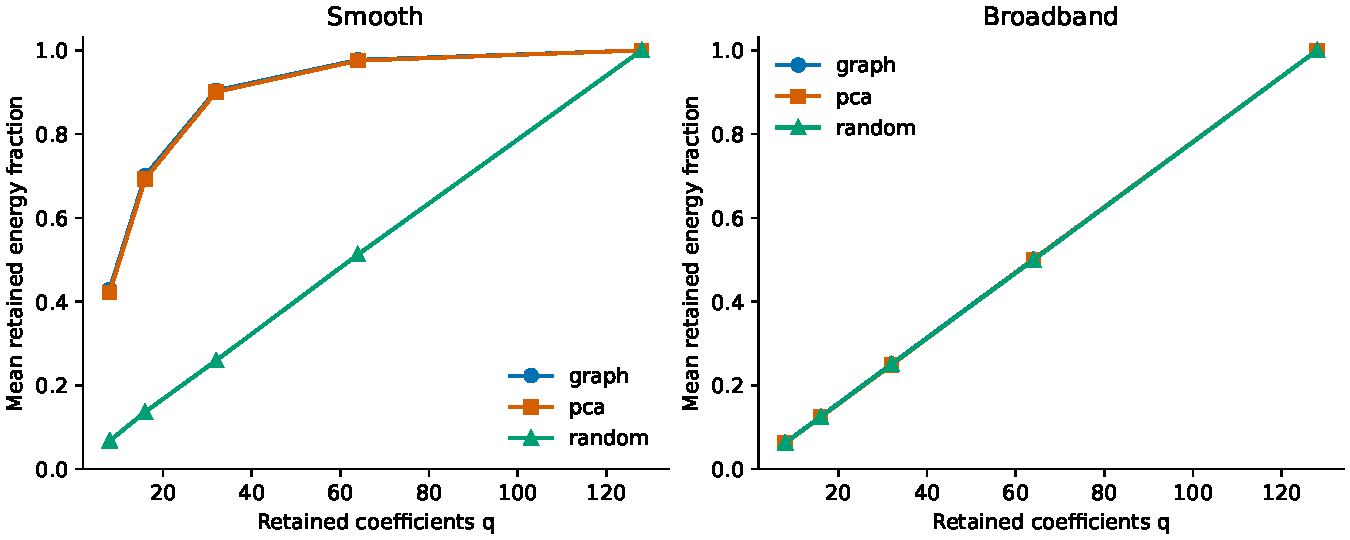
\includegraphics[width=0.94\linewidth]{v2-results/encoding-quality.pdf}
 \caption{Measured retained signal energy across all five coefficient
 budgets. Smooth data are generated in the graph basis with decreasing
 variances; broadband data have isotropic covariance. Lines connect
 tested ranks and do not imply measurements between them.}
 \label{fig:encoding}
\end{figure}

On smooth signals at rank 16, graph encoding retains 70.03\% of the
signal energy, compared with 69.31\% for fitted PCA and 13.67\% for the
random basis. The graph MSE is 0.038257, close to its analytical
expectation 0.038144. PCA's paired excess MSE is 0.000997
(95\% interval [0.000845, 0.001153]). At rank 64, graph encoding
retains 97.72\% of energy with MSE 0.002842, while PCA retains 97.53\%
with MSE 0.003074 and the random basis retains 51.25\% with MSE
0.065333. This is the expected behaviour of an oracle-aligned graph
basis, a finite-sample estimate of it, and an unaligned dictionary.

On broadband signals at rank 64, the graph, PCA and random-basis MSEs
are 0.500758, 0.501700 and 0.502710, respectively, around the common
population value 0.5. Both paired intervals relative to graph include
zero. Retained energies are correspondingly near 50\%. All three
full-rank encoders reconstruct to floating-point accuracy; their
minute full-rank differences are numerical residuals, not a compression
advantage. The controls support a distribution-dependent basis
alignment effect, not universal graph compression.

\subsection{Decoding}

Table~\ref{tab:decoding} gives the fixed named arms and the two reference
estimators. Figure~\ref{fig:decoding} retains all 32 phase controls.
Negative changes denote lower error than heat. The paired comparisons
measure the effect of redistribution within the retained chart at
fixed isotropic-noise transmission.

\begin{table}[htbp]
 \centering\small
 \begin{tabular}{llrrl}\toprule
Regime & Arm & MSE & $\Delta$MSE & Paired 95\% interval \\\midrule
smooth & heat & 0.061151 & +0.000000 & [+0.000000, +0.000000] \\
smooth & envelope & 0.061516 & +0.000365 & [+0.000326, +0.000405] \\
smooth & prime & 0.061754 & +0.000603 & [+0.000470, +0.000739] \\
smooth & projection & 0.128377 & +0.067226 & [+0.066568, +0.067881] \\
smooth & noisy & 0.252259 & +0.191109 & [+0.189898, +0.192240] \\
broadband & heat & 0.684918 & +0.000000 & [+0.000000, +0.000000] \\
broadband & envelope & 0.694222 & +0.009305 & [+0.009193, +0.009409] \\
broadband & prime & 0.680581 & -0.004336 & [-0.004479, -0.004181] \\
broadband & projection & 0.625163 & -0.059755 & [-0.061291, -0.058174] \\
broadband & noisy & 0.250873 & -0.434045 & [-0.438254, -0.429528] \\
\bottomrule\end{tabular}

 \caption{Noisy rank-64 reconstruction. $\Delta$MSE is relative to heat;
 intervals are descriptive paired bootstrap intervals. Projection and
 noisy-observation references do not satisfy the heat-family gain-norm
 constraint.}
 \label{tab:decoding}
\end{table}

\begin{figure}[htbp]
 \centering
 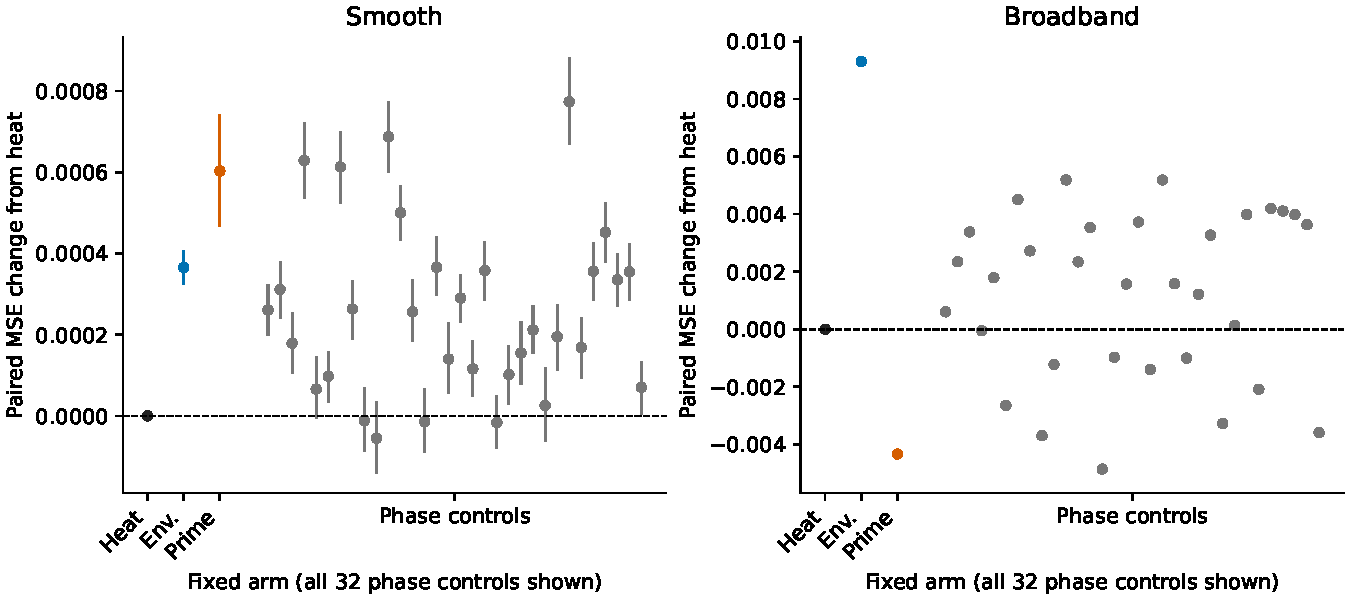
\includegraphics[width=0.94\linewidth]{v2-results/decoding-quality.pdf}
 \caption{Measured paired changes from heat for every fixed modal arm,
 including all phase controls. Vertical bars show descriptive 95\%
 bootstrap intervals. The zero line is the heat reference, not an
 image-quality threshold.}
 \label{fig:decoding}
\end{figure}

The realised shared scale is $\beta=0.0520782$; multipliers range from
0.75 to 1.171732. The heat-family squared gain norm is 26.786642,
with maximum absolute matching residual $7.11\times10^{-15}$.
Thus the reported differences are not explained by a different
expected transmitted isotropic-noise energy.

On smooth signals, prime gating increases MSE from 0.061151 to
0.061754, a paired change of $+0.000603$ with descriptive 95\%
interval $[0.000470,0.000739]$. The envelope also raises MSE, to
0.061516. The phase-control MSE range is
$[0.061096,0.061924]$, and prime ranks 29th among the 33 prime and
phase arms. This is an unfavourable outcome for the prime design in
the population most closely aligned with the low-frequency graph prior.

On broadband signals, prime gating lowers MSE from 0.684918 to
0.680581, a paired change of $-0.004336$ with descriptive interval
$[-0.004479,-0.004181]$. The envelope instead raises MSE to
0.694222. The phase-control range is $[0.680058,0.690107]$ and prime
ranks 2nd of 33: phase-13 performs better, so the finite arithmetic
waveform has no unique advantage even in this favourable regime.
Moreover, unfiltered projection achieves 0.625163 and the full noisy
observation achieves 0.250873. The prime arm's improvement over heat
does not overcome the distortion caused by the chosen rank restriction
and attenuation on broadband data.

The secondary graph-weighted error changes in the same direction
for prime versus heat: from 0.026394 to 0.027046 on smooth data,
and from 1.812352 to 1.808342 on broadband data. The envelope illustrates
why the two outcomes differ: it lowers smooth graph-weighted error
to 0.025599 while increasing ordinary MSE. These are distinct quadratic
losses. Equation~\eqref{eq:risk} explains the general pattern as a
redistribution of signal distortion under different modal variances;
it supplies no theorem selecting the prime waveform.

\subsection{Clock invariance}

\begin{table}[htbp]
 \centering\small
 \begin{tabular}{lrr}\toprule
Steps & Max exact error & Max Euler error \\\midrule
64 & 2.887e-15 & 4.263e-03 \\
256 & 1.366e-14 & 1.062e-03 \\
1024 & 5.462e-14 & 2.651e-04 \\
\bottomrule\end{tabular}

 \caption{Maximum transfer-function errors relative to exact unit-time
 heat evolution. Each entry is the maximum across all prescribed clock
 arms at that resolution; exact evolution and Euler use the same cells.}
 \label{tab:clock}
\end{table}

Across all arms and refinements the largest exact residual is
$5.462\times10^{-14}$. The largest Euler errors decrease from
$4.263\times10^{-3}$ at 64 steps to $1.062\times10^{-3}$ at 256
and $2.651\times10^{-4}$ at 1,024, consistent with first-order
convergence. The exact calculation tests Proposition~2, while the Euler sequence
tests convergence under subdivision of the same clock. Finite
precision can accumulate round-off in a product of exact cell
exponentials; a nonzero floating-point residual is not a violation of
the theorem. Conversely, differences between coarse Euler trajectories
cannot establish that arithmetic modulation changes the exact heat
operator.

\section{Interpretation and limits}
\label{sec:limits}

The encoding and decoding experiments address different interventions.
Encoding changes the retained subspace with clean observations.
Decoding fixes the graph subspace and changes attenuation of noisy
coefficients. An encoding advantage under a deliberately smooth
population cannot be credited to prime gating. A decoding advantage
over unit heat cannot by itself establish that the graph basis was
learned appropriately from a corpus.

The bridge to the neural architecture is specific: both the numerical
filter and \code{ModalGate} implement~\eqref{eq:gains}, and the neural
graph block applies that vector within the same project--gate--lift
pattern. The linear study omits learned channel maps, image losses,
the dispersion-conditioned neural gate, spatial residual paths and
diffusion training. Its measured effects are not estimates of the
complete model's performance. Neural training may compensate for the
fixed gain, ignore it, or interact with it; each possibility requires
measurement.

The imposed index correspondence is another substantive limitation.
The path spectrum is simple and its ordering is unambiguous. On graphs
with repeated eigenvalues, independent gains assigned within a
degenerate eigenspace depend on the chosen basis. Sign flips cancel in
$\Uq\diag(d)\Uq^\top$, but arbitrary rotations inside a degenerate
eigenspace do not when gains differ. A corpus experiment must fix and
record the basis or use identical gains within degenerate blocks.
Different graph sizes, normalisations and spectral densities also
change what a unit heat time represents.

Positive bounded multipliers ensure a well-defined finite operation;
they are not a proof of stable learned dynamics, conservation of clean
signal energy, or superior reconstruction. The RH envelope supplies
one principled shape to test, but RH alone makes no prediction about
image semantics or the optimal gain in~\eqref{eq:risk}. A negative
prime result is therefore informative about this design, not about
RH. A favourable result would likewise motivate replication rather
than support a number-theoretic or physical conclusion.

A decisive image experiment would build the frozen graph and dispersion
vector from training-only corpus embeddings, then train matched spatial
VAEs with and without the constructive graph branch. Heat, envelope,
prime and phase controls would use equal trainable capacity, optimisation
budgets and independently repeated seeds. Evaluation would measure
held-out reconstruction and semantic consistency, including total
latent and chart storage. A second stage would freeze the selected VAE
and train the latent denoiser, with a specified chart source at
generation time. These are proposed experiments, not results of v2.

\section{Reproducibility and implementation boundary}
\label{sec:repro}

The numerical study is implemented in \code{src/ald_sc/prime_gating.py};
\code{scripts/run_prime_study.py} produces the JSON report, per-signal
arrays, figures and the three directly included tables. The local
protocol is \code{docs/experiments/prime-gating-protocol.md}.
The report records configuration, Python and NumPy versions, input-array
hashes, source and lockfile hashes, and the base commit. A base commit
alone does not identify uncommitted work; the recorded file hashes are
part of the numerical provenance.

From the repository root, the numerical artefacts can be generated in
the project's \code{.venv} using:
\begin{verbatim}
uv sync --locked --group notebooks
uv run --locked --group notebooks python scripts/run_prime_study.py
\end{verbatim}
The manuscript is then built from \code{docs/paper} using two passes:
\begin{verbatim}
pdflatex -interaction=nonstopmode -halt-on-error ald-sc-v2.tex
pdflatex -interaction=nonstopmode -halt-on-error ald-sc-v2.tex
\end{verbatim}
The generated tables and figures are included directly.
The file \code{results.json} contains all phase controls;
\code{raw-outcomes.npz} contains paired outcomes and waveform arrays.
The executed notebooks in \code{notebooks/} expose the same operations:
\begin{verbatim}
01-v2-encoding-quality.ipynb
02-v2-prime-decoding.ipynb
\end{verbatim}
To execute both notebooks, use:
\begin{verbatim}
uv run --locked --group notebooks python scripts/execute_v2_notebooks.py
\end{verbatim}

\begin{table}[htbp]
 \centering\small
 \begin{tabular}{p{0.33\linewidth}p{0.58\linewidth}}
 \toprule
 Component & Implementation and evidential role\\
 \midrule
 Frozen graph and chart & \code{arrow_prior.py}: non-trainable geometry,
 chart energies and dispersion projection.\\
 Spatial posterior & \code{vae.py}: dual-head encoder and eagerly
 constructed graph decoder bound to its prior.\\
 Constructive decoding & \code{graph_decoder.py}: learned chart gate
 multiplied by frozen modal gains at three stages.\\
 Modal recipe & \code{modal_gate.py}: heat-matched positive gains and
 checkpoint recipe identity.\\
 Linear experiments & \code{prime_gating.py}: held-out encoding,
 all decoding controls and common-clock errors.\\
 Latent denoising & \code{dit.py}, \code{schedule.py}: spatial-latent
 diffusion; not evaluated by the linear signal experiments.\\
 \bottomrule
 \end{tabular}
 \caption{Code-to-claim mapping for version 2.0.0.}
 \label{tab:code}
\end{table}

This revision preserves the original manuscript as a historical
document. Earlier test counts, toy image outputs and claims of
mode-specific cosine resolution are not used as current experimental
evidence. Software tests establish defined behaviours; the saved
numerical outcomes establish the limited empirical claims made here.

\section*{Availability and acknowledgement}

Source and accompanying artefacts are maintained at:
\par\noindent
\url{https://github.com/tuned-org-uk/arrowspace-latent-diffusion}.
AI-assisted tools supported drafting and implementation review.
Responsibility for the mathematical statements, evidence and final
interpretation remains with the author.

\begin{thebibliography}{9}
\bibitem{rombach}
R.~Rombach, A.~Blattmann, D.~Lorenz, P.~Esser and B.~Ommer.
\newblock High-resolution image synthesis with latent diffusion models.
\newblock In \emph{CVPR}, 2022.
\newblock \url{https://arxiv.org/abs/2112.10752}.

\bibitem{kingma}
D.~P.~Kingma and M.~Welling.
\newblock Auto-encoding variational Bayes.
\newblock arXiv:1312.6114, 2013.
\newblock \url{https://arxiv.org/abs/1312.6114}.

\bibitem{peebles}
W.~Peebles and S.~Xie.
\newblock Scalable diffusion models with transformers.
\newblock arXiv:2212.09748, 2022.
\newblock \url{https://arxiv.org/abs/2212.09748}.

\bibitem{shuman}
D.~I.~Shuman, S.~K.~Narang, P.~Frossard, A.~Ortega and P.~Vandergheynst.
\newblock The emerging field of signal processing on graphs: extending
high-dimensional data analysis to networks and other irregular domains.
\newblock \emph{IEEE Signal Processing Magazine}, 2013.
\newblock \url{https://doi.org/10.1109/MSP.2012.2235192}.

\bibitem{arrowspace}
tuned-org-uk.
\newblock \emph{pyarrowspace}: Python bindings and source for ArrowSpace.
\newblock Software repository, accessed 21 November 2026.
\newblock \url{https://github.com/tuned-org-uk/pyarrowspace}.

\bibitem{schoenfeld}
L.~Schoenfeld.
\newblock Sharper bounds for the Chebyshev functions $\theta(x)$ and
$\psi(x)$. II.
\newblock \emph{Mathematics of Computation}, 30(134):337--360, 1976.
\newblock \url{https://doi.org/10.1090/S0025-5718-1976-0457374-X}.
\end{thebibliography}
\end{document}
